\documentclass{article}

\usepackage{graphicx}
\usepackage{multirow}

\title{Note: Logistic Regression}
\author{Sun Zhao}

\begin{document}
\maketitle
\newpage

\section{Classification}
In classification problem, we will predict the label for the given data instead of continuous values like regression problem. For example, a classifier may automatically label an email as spam or not spam, an online transaction fraudulent or not fraudulent, or a tumor malignant or benign. In the simplest case, there are only two classes. Usually, we use 0 and 1 to denote the negative class and the positive class separately. Figure\ref{classification_example} shows a training data set of tumor classification. When using linear regression algorithm and exclude blue cross example, we get a hypothesis of purple line. Naturally, we define 0.5 as the boundary of malignant or benign, ie, if the hypothesis h(x) is equal to or greater than 0.5, then x is malignant, otherwise benign. Let $h(x_{0})$ = 0.5, then if x >= $x_{0}$, x is malignant, otherwise benign. In this case, we get a perfect classifier. However, if the blue cross is included, we may get a hypothesis of green line. And let $h(x_{1})$ = 0.5, obviously, $x_{1}$ is worth than $x_{0}$ when classifying tumors. This is because in the binary classification problem, the value of y is always 0 or 1, but the output of linear regression can be larger than 1 or smaller than 0. Logistic regression will use a hypothesis $h_{\theta}(x)$ whose output is always between 0 and 1.

\begin{figure}[ht]
  \centering
  % Requires \usepackage{graphicx}
  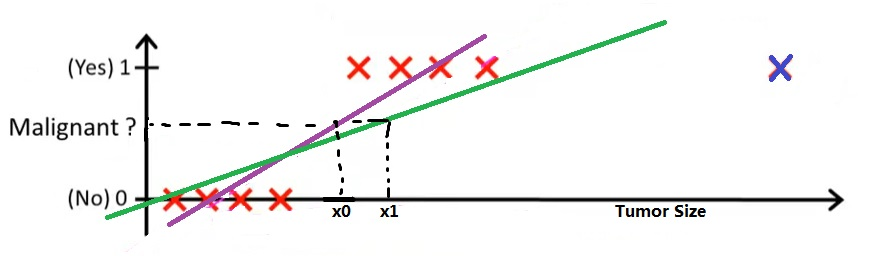
\includegraphics[width=8cm]{Figure1.jpg}\\
  \caption{}\label{classification_example}
\end{figure}

\section{Hypothesis Representation}
How to control the output of our hypothesis between 0 and 1? The answer is using a sigmoid function shown in (\ref{sigmoid_function}). The sigmoid function plotted in Figure\ref{sigmoid_function_plotting} maps an interval of (-$\infty, \infty$) to (0, 1). Combining the sigmoid function and hypothesis function $h_{\theta}(x) = \theta^{T}x$, we will get the hypothesis function of logistic regression shown in (\ref{logistic_regression_hypothesis}). The output of the new hypothesis $h_{\theta}(x)$  means the probability that y = 1 on input of x. For example, in the tumor classification problem, if $h_{\theta}(x_{0}) = 0.7$, then we can tell the patient whose tumor size is equal to $x_{0}$ that there are 70\% chance that her/his tumor to be malignant. Formally, the hypothesis predicts the probability of x being positive class given x and $\theta$. This definition is described in (\ref{hypothesis_probability_definition}), and obviously, we can induce a property shown in (\ref{probalility_property}).
\begin{equation}\label{sigmoid_function}
Sigmoid(x) = \frac{1}{1 + e^{-x}}
\end{equation}

\begin{equation}\label{logistic_regression_hypothesis}
h_{\theta}(x) = \frac{1}{1 + e^{-\theta^{T}x}}
\end{equation}

\begin{equation}\label{hypothesis_probability_definition}
h_{\theta}(x) = P(y = 1|x;\theta)
\end{equation}

\begin{equation}\label{probalility_property}
P(y = 0|x;\theta) + P(y = 1|x;\theta) = 1
\end{equation}

\begin{figure}[ht]
  \centering
  % Requires \usepackage{graphicx}
  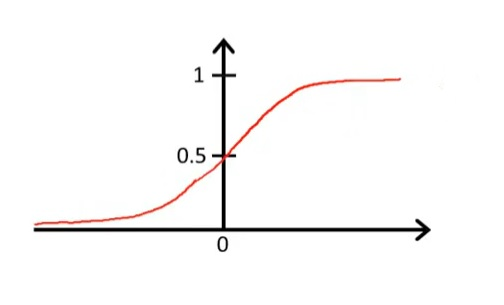
\includegraphics[width=8cm]{Figure2.jpg}\\
  \caption{}\label{sigmoid_function_plotting}
\end{figure}

\section{Decision Boundary}
Because we judge a sample x whether is positive class by checking whether its hypothesis value $h_{\theta}(x)$ equal to or greater than 0.5, and note Sigmoid(0) = 0.5, we can use the condition that whether $\theta^{T}x$ is equal to or greater than 0 to decide its class. If we plot the examples and hypothesis function when given $\theta$, we will find that $\theta^{T}x$ = 0 defines the decision boundary between two classes. Figure\ref{decision_boundary} shows two decision boundaries. In Figure\ref{decision_boundary}A, all positive examples are from the up-right direction of the decision line, and in Figure\ref{decision_boundary}B, they are all from the outside direction of the decision circle.

\begin{figure}[ht]
  \centering
  % Requires \usepackage{graphicx}
  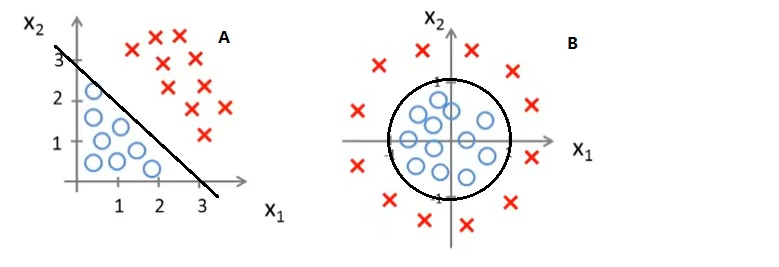
\includegraphics[width=8cm]{Figure3.jpg}\\
  \caption{}\label{decision_boundary}
\end{figure}

\section{Cost Function}
Now we have the logistic regression hypothesis shown in (\ref{logistic_regression_hypothesis}), if we use square error cost function as linear regression, the cost function is much complicated and non-convex, hence the gradient descent algorithm may not converge with a global optima. To ensure a convex cost function, we define the cost between $h_{\theta}(x)$ and y as $Cost(h_{\theta}(x), y)$ shown in (\ref{logistic_regression_example_cost_function}).

\begin{equation}\label{logistic_regression_example_cost_function}
Cost(h_{\theta}(x), y) = \left\{ \begin{array}{ll}
-log(h_{\theta}(x)) & \textrm{if y = 1}\\
-log(1 - h_{\theta}(x)) & \textrm{if y = 0}\\
\end{array} \right.
\end{equation}
The intuition behind the cost function is that if $h_{\theta}(x) = 0$, but y = 1 or $h_{\theta}(x) = 1$, but y = 0, we'll penalize learning algorithm by a very large cost, and if $h_{\theta}(x)$ = y, the cost is zero. Figure\ref{cost_fuction_log_plot} shows $-log(h_{\theta}(x))$ against $h_{\theta}(x)$ (when y = 1, the cost function will be $-log(h_{\theta}(x)$), and it is clear that the cost decreases as $h_{\theta}(x)$ goes 1.
\\
Since y only equal 1 or 0, we can refine $Cost(h_{\theta}(x), y)$ in a simple form shown in (\ref{simple_logistic_regression_example_cost_function}).

\begin{figure}[ht]
  \centering
  % Requires \usepackage{graphicx}
  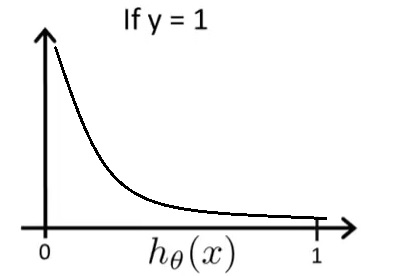
\includegraphics[width=5cm]{Figure4.jpg}\\
  \caption{}\label{cost_fuction_log_plot}
\end{figure}

\begin{equation}\label{simple_logistic_regression_example_cost_function}
Cost(h_{\theta}(x), y) = -ylog(h_{\theta}(x)) - (1 - y)log(1 - h_{\theta}(x))
\end{equation}
\\
Thus, the cost function of logistic regression becomes (\ref{logistic_regression_cost_function}).
\begin{eqnarray}\label{logistic_regression_cost_function}
% \nonumber to remove numbering (before each equation)
  J(\theta) &   =   &\frac{1}{m} \sum_{i=1}^{m} Cost(h_{\theta}(x^{(i)}), y^{(i)})\\
            &   =   &-\frac{1}{m} \sum_{i=1}^{m} y^{(i)}log(h_{\theta}(x^{(i)})) + (1 - y^{(i)})log(1 - h_{\theta}(x^{(i)}))
\end{eqnarray}

\section{Gradient Descent}
According to cost function shown in (\ref{logistic_regression_cost_function}) and gradient descent idea, we get the gradient descent algorithm for logistic regression. Algorithm1 shows the update iteration, and it is cool that the update function looks identical with linear regression! The only difference is the hypothesis function.
\smallskip
\hrule
\smallskip
Algorithm1: Gradient Descent for Logistic Regression
\smallskip
\hrule
\smallskip
Repeat\{\\
$\theta_j=\theta_j - \alpha \frac{1}{m} \sum_{i=1}^{m}(h_\theta(x^{(i)})-y^{(i)}) \cdot x^{(i)}_{j}$\\
\}\\
\hrule

\section{Multiple Class Classification}
Contrasting with binary classification, multiple class classification predicts more than two classes. Here are a list of examples:
\begin{itemize}
\item Email tagging: Work, Friends, Family.
\item Medical diagrams: Not ill, Cold, Flu.
\item Weather: Sunny, Cloudy, Rain, Snow.
\end{itemize}
The idea of One-vs-All is to train a binary logistic regression classifier $h_{\theta}^{(c)}(x)$ for each class c(treat examples belonging to c as positive class and examples not belonging to class c as negative class) to predict the probability that x is a member of class c. On a new input of x, its class is predicted as c that maximize $h_{\theta}^{(c)}(x)$.

\section{Summary}
Logistic regression solves the classification problem. When using a sigmoid like hypothesis and logarithms cost function, the update iteration is identical to linear regression except the hypothesis. Multiple binary classifiers are trained for each class when solving multiple class classification problem.
\end{document}
